% 2019_shanghai_spring_q17_fig1: regular triangular pyramid P-ABC, M on PB, N on BC
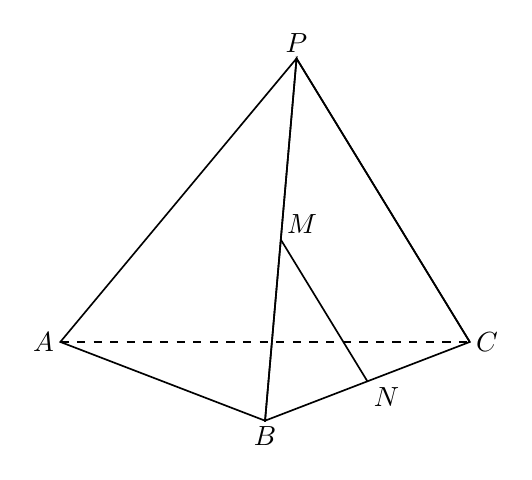
\begin{tikzpicture}[x=1cm,y=1cm,font=\normalsize,line width=.6pt,
  geometry edge/.style={draw=black,solid,line width=.6pt},
  geometry hidden/.style={draw=black,dashed,line width=.6pt},
  geometry label/.style={font=\normalsize,inner sep=2pt}]
\coordinate (P) at (3.0,4.6);
\coordinate (A) at (0,1.0);
\coordinate (B) at (2.6,0);
\coordinate (C) at (5.2,1.0);
\coordinate (M) at (2.8,2.3);
\coordinate (N) at (3.9,0.5);
\draw[geometry edge] (P)--(A)--(B)--cycle;
\draw[geometry edge] (P)--(B)--(C)--cycle;
\draw[geometry edge] (P)--(C);
\draw[geometry edge] (M)--(N);
\draw[geometry hidden] (A)--(C);
\node[geometry label,above] at (P) {$P$};
\node[geometry label,left] at (A) {$A$};
\node[geometry label,below] at (B) {$B$};
\node[geometry label,right] at (C) {$C$};
\node[geometry label,above right] at (M) {$M$};
\node[geometry label,below right] at (N) {$N$};
\end{tikzpicture}
